\chapter{Related Work}
\label{chapter:related-work}
 
The hypothesis of Chapter~\ref{chapter:introduction} draws on four bodies of work that have
developed largely apart from one another. Network neuroscience supplies the connectome and
the standards by which claims about its structure are judged. Reservoir computing supplies a
way of holding a wiring diagram fixed while something is asked of it. Random-matrix theory
describes what the spectrum of such a matrix looks like and what that spectrum determines.
A literature on the geometry of neural population activity supplies the vocabulary in which
the consequences are measured. This chapter takes them in that order. Its purpose is not to
survey any of them, but to assemble the minimum each contributes: enough to see why the
hypothesis is worth testing, and enough vocabulary to follow the chapters that test it.
 
 
\section{Brain networks and their null models}
\label{section:brain-networks}
\bigskip
 
Network neuroscience treats a nervous system as a graph and asks what its structure
implies for its function \cite{bassett2017network}. Sporns et al. \cite{sporns2005human}
introduced the term \emph{connectome} for a comprehensive, time-invariant description of
the connections of a nervous system, conceived as a connection matrix whose entries can be
successively annotated with direction, sign and conduction delay. Empirical maps now exist
across scales, from macroscale tract networks reconstructed from diffusion imaging
\cite{sporns2011human, griffa2019structural} to single-cell reconstructions of invertebrate
nervous systems \cite{cook2019whole, dorkenwald2024neuronal}. The apparatus built on
them, which describes a network through its degree distribution, clustering, modularity
and hub structure (Figure~\ref{fig:network-neuro}), is the vocabulary in which the question
of this thesis is posed: asking whether biological connectivity confers computational
advantage is, in the first instance, a question about which features of a wiring diagram
carry weight.
 
\begin{figure}[ht]
    \centering
    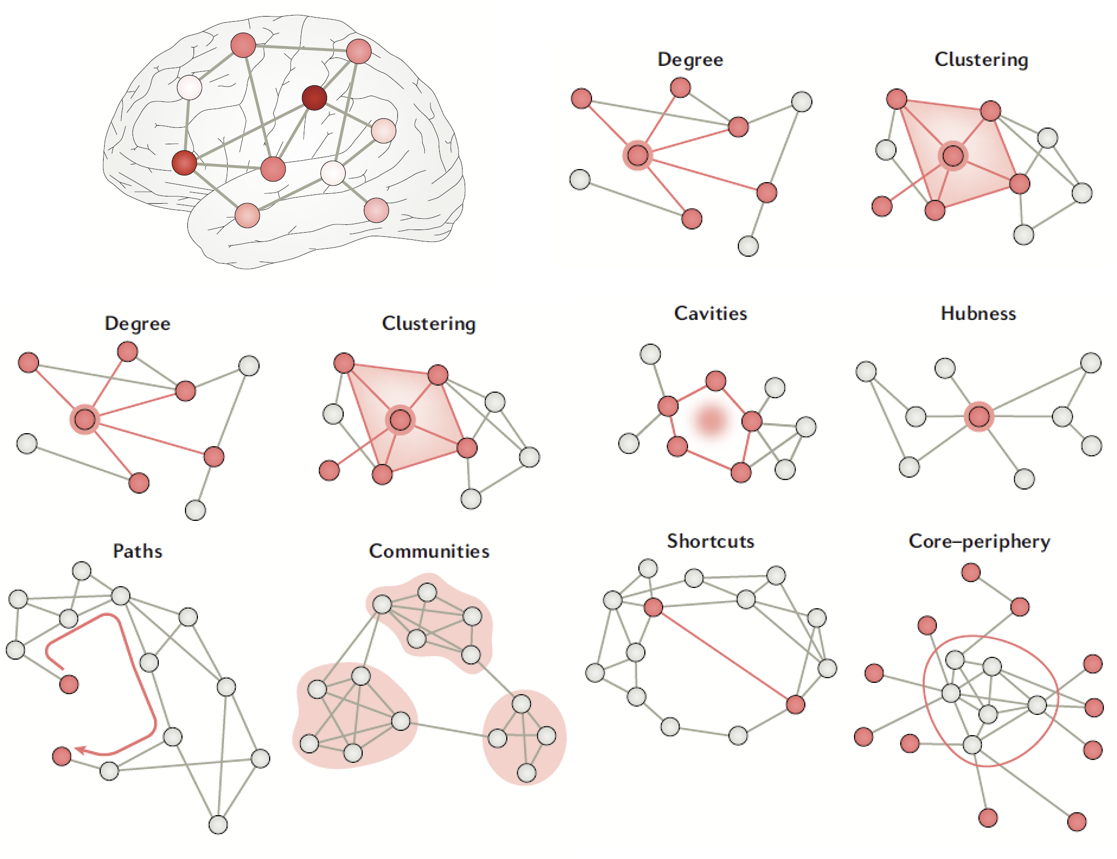
\includegraphics[width=\textwidth]{figures/NetworkNeuro.png}
    \caption[Schematic of network models used in neuroscience]
    {\textbf{Schematic of network models used in neuroscience}.
    A network is characterised through measures such as \emph{degree}, the number
    of edges at a node; \emph{clustering}, the prevalence of triangles;
    \emph{communities}, groups of densely interconnected nodes; and \emph{hubness},
    a node's influence over the rest of the network. Also shown are paths,
    shortcuts, cavities and core-periphery structure.
    (Figure adapted from \cite{bassett2018nature})}
    \label{fig:network-neuro}
\end{figure}
 
The field's most consistent methodological commitment is that a structural claim is only
as credible as the null model it is compared against. What began as a methodological
aside \cite{bassett2017network} has become a validity criterion \cite{bassett2018nature},
the subject of a review in its own right \cite{vavsa2022null}, and a standard extended to
models of signal propagation \cite{seguin2023brain}. Váša and Mišić \cite{vavsa2022null}
set out a graded spectrum of nulls, running from liberal Erdős-Rényi randomisation through
degree-preserving rewiring to spatially and cost-constrained variants, and argue that
comparison against such a spectrum is how the contributions of distinct features are
separated from one another. This is the idea the thesis's null-model ladder
operationalises.
 
Two observations make a graded ladder necessary rather than merely thorough. The first is
that what counts as non-random depends on the null chosen. Small-worldness, modularity and
rich-club structure are treated as robust regularities \cite{bassett2017network}, yet
several dissolve under degree-preserving rewiring \cite{vavsa2022null}, and small-worldness
as canonically defined presupposes shortest-path signalling that is biologically
implausible \cite{seguin2023brain}. The second is that features induce one another as
byproducts: modules and hubs together generate rich-club structure even when neither was
the operative driver \cite{vavsa2022null}. Attributing an effect to a single feature
therefore means separating it from the features it correlates with by construction
\cite{bassett2018nature, suarez2020linking}.
 
A further finding motivates treating the connectome dynamically rather than descriptively.
Roughly half the variance in functional connectivity is unexplained by direct structural
connectivity \cite{suarez2020linking, seguin2023brain}, because functional interactions
reflect polysynaptic, higher-order processes that only an explicit model of signal
propagation can recover. A reservoir, in which input history is transformed by repeated
propagation through fixed recurrent connections, is a model of exactly this kind, and
Suárez et al. \cite{suarez2020linking} identify reservoir computing in this role directly,
citing the connectome-reservoir work of Kawai et al. \cite{kawai2019small}.
 
How much of function structure alone can account for remains contested. Bargmann and
Marder \cite{bargmann2013connectome} argue that even the complete C. elegans connectome has
been largely uninformative about which connections drive specific behaviours, because
parallel pathways, neuromodulatory reconfiguration and intrinsic neuronal dynamics together
let one anatomical wiring support many functional outputs. Recent work shifts the balance
back: Vishwanathan et al. \cite{vishwanathan2024predicting} insert a synapse-resolved
zebrafish brainstem connectome directly as the weight matrix of a linear rate model and
reproduce population-level coding properties measured in separate animals. Their model
fails, however, without an excitatory-inhibitory sign assignment by cell type. The question
is therefore not whether structure can predict function but how much non-structural detail
is the minimum needed, and sign is the first item on that list. It is also the first
property this thesis varies.
 
What this literature does not do is follow its own suggestion. Reservoir computing is named
as the kind of propagation model these reviews call for, and then mentioned with substance
exactly once across them; nulls preserving sign or excitatory-inhibitory balance are barely
treated at all. The next section takes the suggestion up and asks what happens when the
reservoir's connectivity is a connectome.
 
 
 
 
\section{Connectome-constrained reservoirs}
\label{section:connectome-reservoirs}
\bigskip
 
Section~\ref{section:ch2_3} set out the reservoir architecture and what it buys. Because
the recurrent weights are never trained, a difference in performance between two reservoirs
is attributable to the wiring they were given \cite{jaeger2001echo, maass2002real,
yan2024emerging}, and it is this property that has made the framework attractive for
biological connectivity. One convention travels with it. The recurrent matrix is routinely
rescaled so that its spectral radius sits near the boundary of fading memory
\cite{tanaka2019recent, soussia2026reservoir}, which for a random matrix is housekeeping.
For a connectome, whose spectral radius is set by its own weights and topology, it is an
editorial choice about which feature of the substrate to preserve. The thesis treats it as
a variable rather than a step.
 
Reservoir computing's own literature has rarely put a real wiring diagram in the recurrent
matrix. Jaeger's reservoir is randomly sparse, and he is explicit that the topology was an
ad hoc choice \cite{jaeger2001short}; Yan et al. \cite{yan2024emerging} name structured
non-random graphs as an underexplored direction; Tanaka et al. \cite{tanaka2019recent}
survey biological reservoirs in which the biology lies in the dynamics rather than in the
topology; and Soussia et al. \cite{soussia2026reservoir}, the closest methodological
neighbour, feed brain graphs into a graph convolution whose reservoir weights are
themselves random. Whether the substrate contributes anything is not settled even in
principle: Gauthier et al. \cite{gauthier2021next} replace an entire reservoir with a
nonlinear vector autoregression over a handful of recent inputs on standard chaotic
benchmarks, with no loss. What decides the question is a bound on how much a fixed-size
network can hold, and Section~\ref{section:spectra-capacity} returns to it.
 
\begin{figure}[h!]
    \centering
    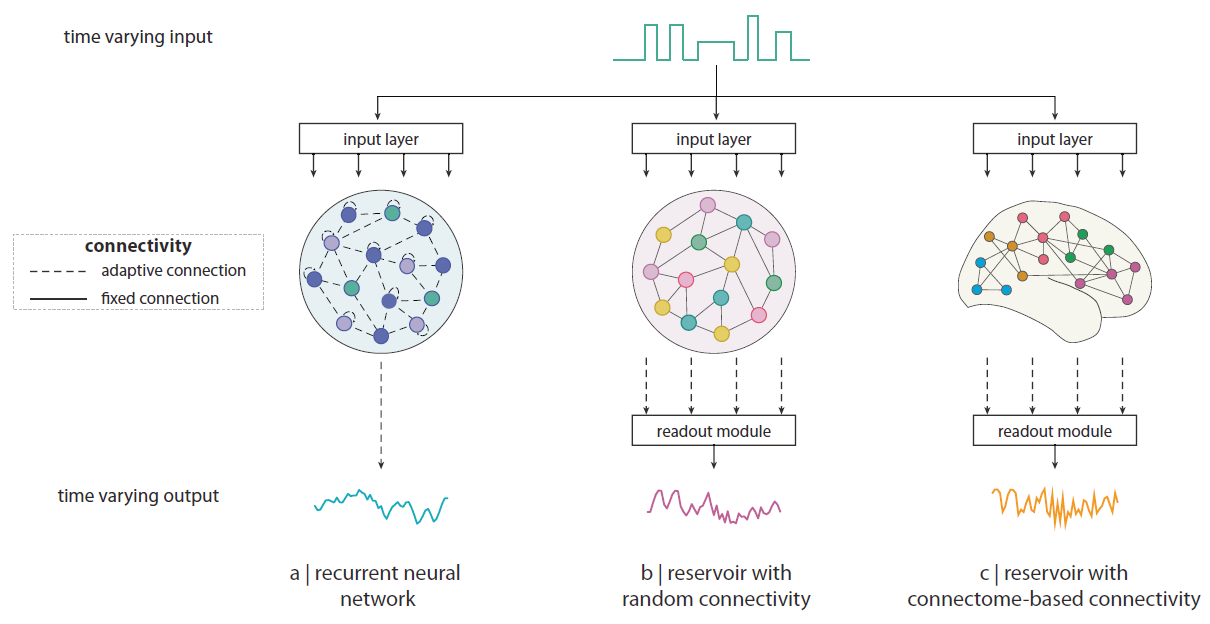
\includegraphics[width=1\textwidth]{figures/Evolution_of_RC.png}
    \caption[Towards connectome-based connectivity in recurrent neural networks]{
    \textbf{Towards connectome-based connectivity in recurrent neural networks}.
    \textbf{(a)} In a classic recurrent neural network the recurrent connections are
    learned, and the topology that emerges from training need not resemble biological
    connectivity.
    \textbf{(b)} In conventional reservoir computing the recurrent weights are assigned
    randomly and held fixed, with learning confined to the readout.
    \textbf{(c)} Advances in imaging now allow the reservoir to be built directly from
    empirical structural connectivity.
    (Figure taken from \cite{suarez2024connectome})}
    \label{fig:connectome-constrained-networks}
\end{figure}
 
The work that does supply a real wiring diagram divides into two paradigms. A reservoir
paradigm \cite{damicelli2022brain, suarez2021learning, suarez2024connectome,
costi2025drosophila} fixes the connectome as a non-trainable recurrent matrix and trains
only a linear readout, which licenses attribution of any difference to topology. A
task-optimised paradigm \cite{lappalainen2024connectome, beiran2025prediction,
achterberg2023spatially} fixes biological structure but trains the network's parameters
end to end, buying stronger absolute performance at the cost of confounding structure with
what training made of it. This thesis sits in the first.
 
Within the reservoir paradigm the headline claims appear to disagree, and reconcile through
the dynamical operating point. Damicelli et al. \cite{damicelli2022brain} find no advantage
of a primate cortical connectome over random-topology controls on memory capacity at a
fixed canonical spectral radius. Suárez et al. \cite{suarez2021learning} find that a human
consensus connectome exceeds a degree-preserving rewire at criticality and underperforms it
in the stable and chaotic regimes, a result extended across species through the conn2res
toolbox \cite{suarez2024connectome}. Costi et al. \cite{costi2025drosophila} recover the
same regime structure on a forecasting task, a Drosophila reservoir beating its
random-topology control near spectral radius one and losing to it below. The connectome's
contribution is therefore a function of the state the network is in rather than a fixed
property of the wiring, and a claim that connectomes help is uninterpretable without a
regime attached. That the pattern appears on prediction as well as retention suggests it is
not confined to memory tasks.
 
The null ladders these papers deploy differ in ways that matter. Damicelli et al.
\cite{damicelli2022brain} compare against a topology-randomised control that does not
preserve degree; Suárez et al. \cite{suarez2021learning, suarez2024connectome} use a
degree-and-density-preserving Maslov-Sneppen rewire; Costi et al.
\cite{costi2025drosophila} add an orthogonal decomposition, substituting connectome
topology with random weights and random topology with connectome weights, but their null
bundles all topological structure together rather than isolating single features. None of
the four preserves clustering or modularity independently of degree, which is the rung this
thesis's ladder adds and which Chapter~\ref{chapter:methods} describes in detail. It is the
field-level commitment of Section~\ref{section:brain-networks}, after Váša and Mišić
\cite{vavsa2022null}, that makes this an addition rather than an embellishment.
 
The task-optimised camp returns a contested verdict on whether a connectome and a task
together determine function. Lappalainen et al. \cite{lappalainen2024connectome} train a
mechanistic model of the fly optic lobe on optic-flow estimation and recover the contrast
preference and direction selectivity of dozens of cell types without any neural-activity
supervision, with ablations identifying synapse sign as one of the two critical structural
features. Beiran and Litwin-Kumar \cite{beiran2025prediction} reach the opposite conclusion
at single-neuron resolution, finding the problem generically underdetermined unless
constrained by observed activity. The two differ in the resolution at which they ask the
question rather than in their answer to it.
 
What none of this work does is manipulate weight sign as a control variable, or offer an
account of \emph{why} a biological substrate helps that is stated in terms of the network's
activity rather than its anatomy. The advantage is attributed throughout to modularity, to
criticality, to degree heterogeneity or to spectral-radius tuning. Supplying such an
account, and treating sign as a first-class variable alongside topology, is the territory
this thesis occupies. The two sections that follow assemble what it needs.
 
 
 
 
\section{Spectra, sign and memory capacity}
\label{section:spectra-capacity}
\bigskip
 
The division of a spectrum into a leading eigenvalue and a bulk, which
Section~\ref{section:ch2_2} introduced as a way of reading a connectivity matrix, is not an
ad hoc reading of a scatter plot. It is what random-matrix theory predicts. The eigenvalues
of a large matrix with independent zero-mean entries fill a disc \cite{girko1985circular},
deformed into an ellipse when reciprocal pairs are correlated \cite{sommers1988spectrum},
and the radius of that disc sets the transition to chaos in a randomly connected network
\cite{sompolinsky1988chaos, kadmon2015transition}. Rajan and Abbott
\cite{rajan2006eigenvalue} supply the result the thesis leans on most directly: giving the
weight distribution a nonzero mean leaves the bulk density unchanged and adds a single
outlying eigenvalue. Ahmadian et al. \cite{ahmadian2015properties} generalise this to
arbitrary structured-plus-random matrices, and Tao \cite{tao2013outliers} establishes when
such an outlier survives and when a row-sum condition removes it. A non-negative matrix is
the extreme case of a nonzero mean, and its outlier is the Perron root met in
Section~\ref{section:ch2_2} \cite{horn2012matrix}. The outlier and the bulk are therefore
separate objects with separate causes, which is why they can be manipulated separately.
 
What such an outlier does to activity has been characterised directly. Landau and
Sompolinsky \cite{landau2018coherent} show that a rank-one component which sums activity
over one mode and feeds it back along another drives a network toward a low-dimensional,
spatially coherent state when the two modes overlap, while chaos survives when they are
orthogonal; Mastrogiuseppe and Ostojic \cite{mastrogiuseppe2018linking} develop the
low-rank-plus-random case more generally. This is the closest existing description of what
a non-negative connectome's dominant mode does to the activity beneath it. These are
results about ensembles, however, not about empirical matrices, and the contribution of
this thesis on the spectral side is an empirical instantiation rather than new theory.
 
Against that spectral picture sits a bound on what any such network can hold. Jaeger
\cite{jaeger2001short} defines the short-term memory capacity of an echo state network as
the summed squared correlation between a delayed input and its best linear reconstruction,
and shows that for i.i.d. inputs read out linearly this capacity cannot exceed $N$, the
number of units, with the bound attained when the state variables are linearly independent.
Dambre et al. \cite{dambre2012information} generalise the result from delayed inputs to any
orthonormal basis of functions, giving a total capacity that equals the number of linearly
independent state variables for any system with fading memory. The bound has a consequence
the thesis works within throughout: a connectome and every null on the ladder have the same
$N$ and compete for the same ceiling, so a biological advantage cannot be an increase in
capacity and must instead be a difference in how that fixed budget is allocated. It also
answers the challenge of Gauthier et al. \cite{gauthier2021next} in principle if not in
practice, since what a recurrent state offers beyond a polynomial of recent inputs is
precisely the number of independent directions it makes available.
 
Which spectral property drives that number is less settled. Non-normality is the
established answer. Ganguli et al. \cite{ganguli2008memory} show that the total Fisher
memory of a normal connectivity matrix is fixed regardless of its eigenvalues, and that the
bound is approached only by strongly non-normal, effectively feedforward architectures;
White et al. \cite{white2004short} reach a related conclusion for orthogonal networks,
Toyoizumi and Abbott \cite{toyoizumi2011beyond} for amplification beyond the edge of chaos,
and Orhan and Pitkow \cite{orhan2020improved} demonstrate the effect in trained recurrent
networks. Non-normality is therefore not available to this thesis as a novel explanation,
and it is in any case not available as an explanation at all: the macroscale connectome is
symmetric by construction, so the matrix studied here is normal and its eigenvectors are
orthogonal (Section~\ref{section:ch2_2}). Whatever distinguishes it from a null of the same
size has to be visible in the eigenvalues themselves.
 
One study relates the shape of an eigenvalue distribution to memory directly, and points
the other way. Aceituno et al. \cite{aceituno2020tailoring} report that reservoirs whose
eigenvalues are concentrated near the origin have lower memory capacity than those whose
eigenvalues are spread uniformly, the mechanism being that a larger average modulus
decorrelates unit activity. Read carelessly this contradicts the account developed here.
The two claims concern different objects. Their variable is the radial spread of the whole
distribution, varied by construction; the quantity at issue in this thesis is the
separation between a leading eigenvalue and a bulk whose radius is near-identical across
the networks being compared, so the distributions differ in where the outlier sits rather
than in how far the bulk extends. Their readout is also unregularised, so a direction
counts only insofar as it decorrelates the raw state, whereas a ridge readout credits
directions in proportion to how their variance compares with the regularisation. What
counts as a usable direction is not the same measurement in the two settings. A separate
result on modularity and memory in reservoirs, sometimes conflated with this one, concerns
an intermediate optimum reached through diffusion in threshold units and makes no claim
about eigenvalue shape at all \cite{rodriguez2019optimal}.
 
Weight sign enters this literature as a control on dynamics rather than as a variable under
which structural effects are measured. Krauss et al. \cite{krauss2019weight} identify the
balance between excitation and inhibition as the essential control parameter of a recurrent
network, driving it between oscillatory, chaotic and fixed-point behaviour, with connection
density a far weaker influence; Cornford et al. \cite{cornford2021learning} show that
networks obeying Dale's principle can be trained to match unconstrained ones. Srinivasan et
al. \cite{srinivasan2025boosting} bring the same variable to reservoirs, reporting best
performance at balance or slight over-inhibition and substantial gains from locally
adapting it. That sign gates dynamical regime is established, then, and it is reproduced
here rather than discovered. The question this thesis puts to sign inverts the usual
direction of interest: not which composition performs best, but at what composition a
network's topology stops making any difference at all.
 
 
 
 
\section{Computation through neural population dynamics}
\label{section:geometry}
\bigskip
 
The step from dynamics to computation is usually taken through geometry. A population's
activity over time traces a trajectory through a high-dimensional state space, and
describing the shape of that trajectory has become a standard way of relating neural
dynamics to the computations they support \cite{chung2021neural, vyas2020computation,
ju2020dynamic} (Figure~\ref{fig:neuraldynamics}). The first question asked of such a shape is how many dimensions it occupies,
since a readout confined to few directions has correspondingly little to combine.
 
How connectivity sets that number is an active question. Recanatesi et al.
\cite{recanatesi2019dimensionality} trace the dimensionality of activity in recurrent
spiking networks to local features of connectivity; Hu and Sompolinsky
\cite{hu2022spectrum} derive the covariance spectrum of randomly connected linear networks;
Dahmen et al. \cite{dahmen2019second} relate wide dynamical repertoires to proximity to an
instability; Litwin-Kumar et al. \cite{litwin2017optimal} identify a connectivity degree
that maximises dimension in feedforward expansions; and stimuli \cite{mazzucato2016stimuli}
and learning \cite{farrell2022gradient} both reshape it. Two results bear most closely on
this thesis. Clark et al. \cite{clark2023dimension} give the dimension of activity in random
networks, and in later work \cite{clark2025connectivity} show that it depends on just two
properties of the coupling matrix, its variance and its effective rank.

That last result makes a terminological distinction necessary, since three different objects
in this literature are called a dimension or a rank. The effective rank of the coupling
matrix $\mathbf{W}$ counts the dominant rank-one components of the connectivity
\cite{clark2025connectivity}. The participation ratio of the activity covariance counts the
directions in which the trajectory varies most, weighting each by its variance
\cite{gao2017theory}. The measure used in this report is neither: it is the effective rank
of the state Gram matrix under ridge regularisation, which counts the directions a
particular readout can actually use. The three coincide only in special cases, and the
distance between the second and the third is one of the report's findings.

\begin{figure}[ht]
    \centering
    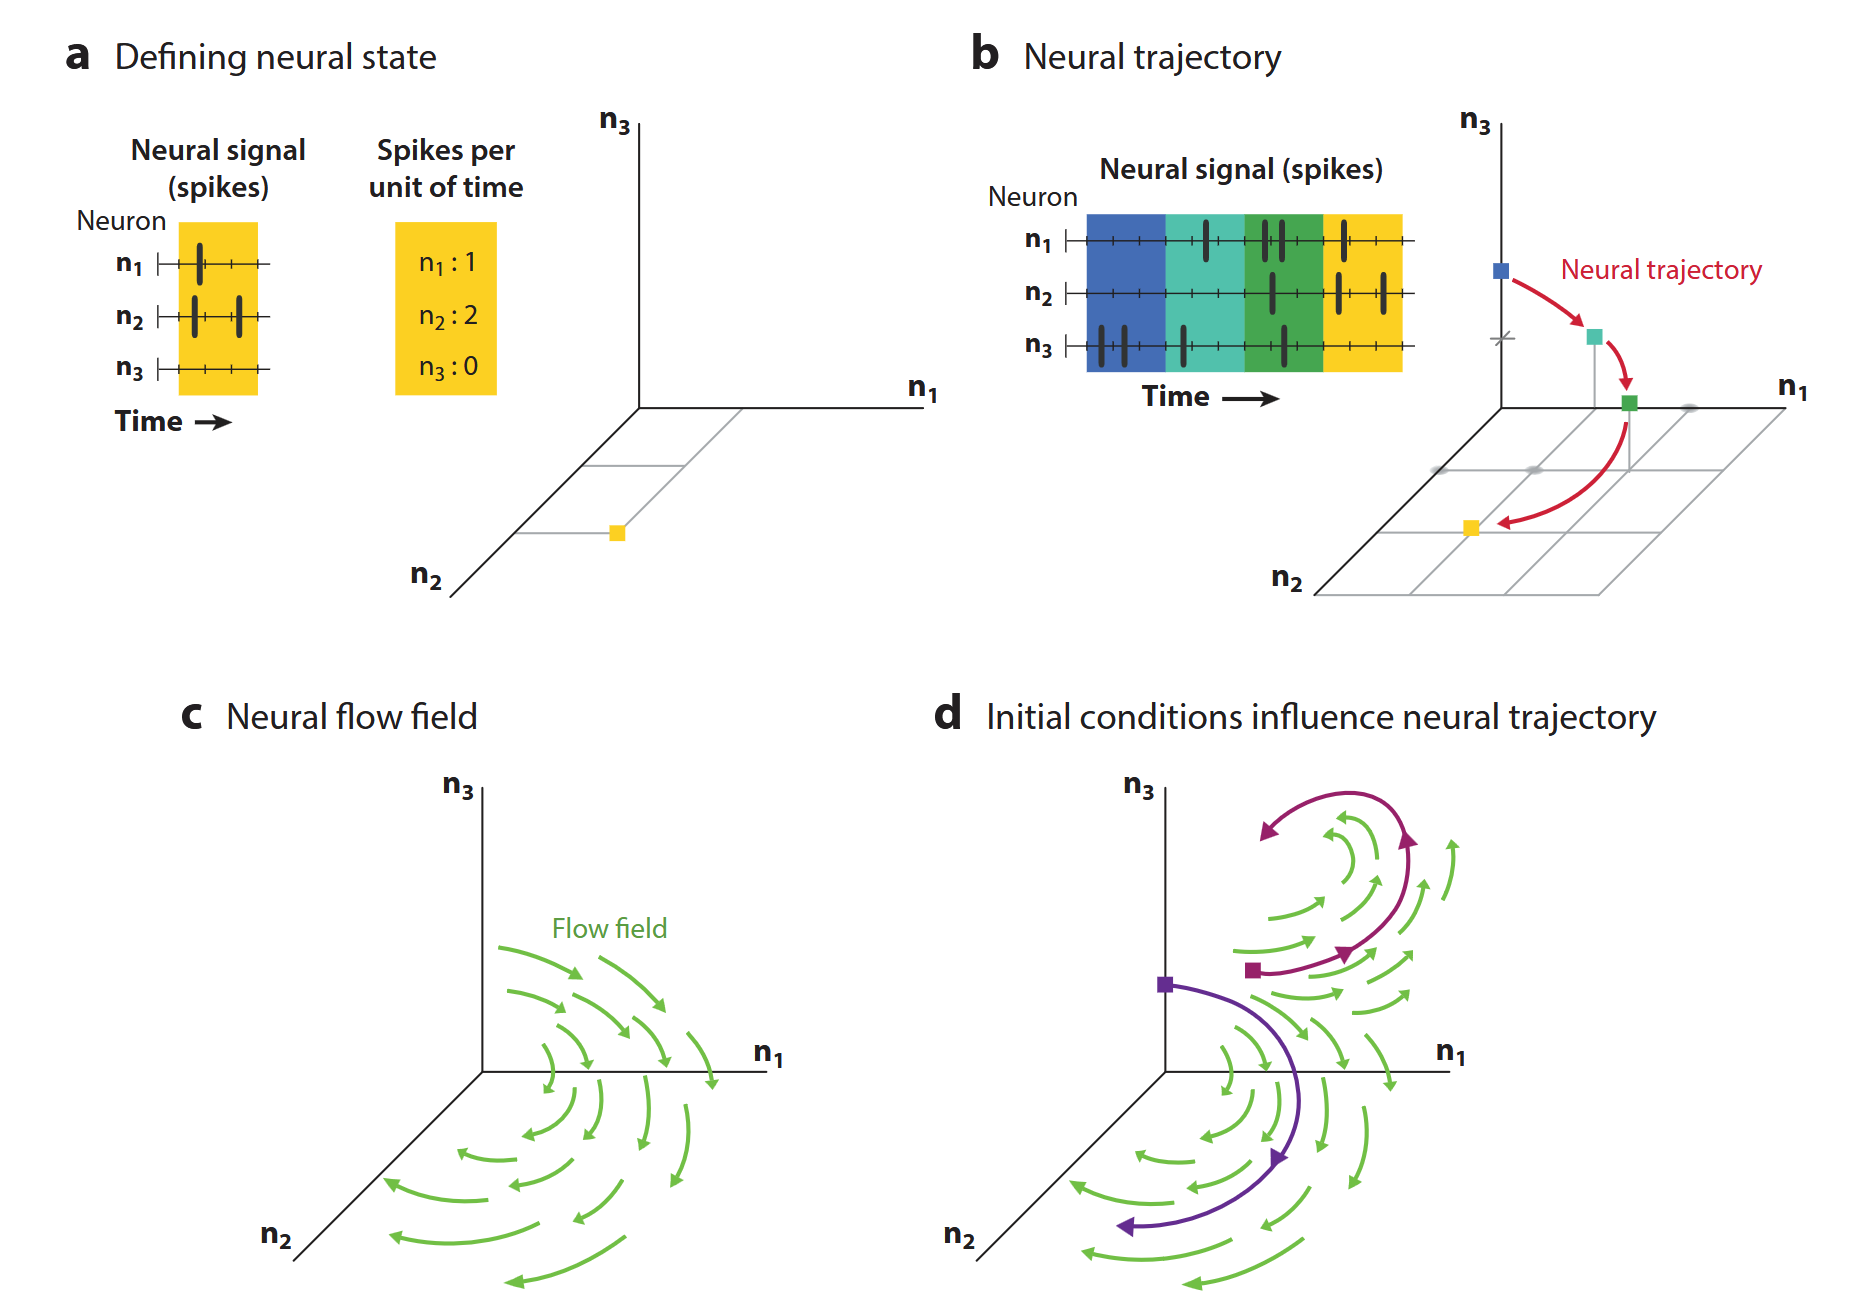
\includegraphics[width=1\textwidth]{figures/NeuralDynamicsSchematic.png}
    \caption[Neural population dynamics and geometry]{
    \textbf{Neural population dynamics and geometry}.
    \textbf{(a, b)} Spikes from three neurons are binned and counted through time, and
    each bin is plotted as a point in a state space whose axes are the three neurons
    (n1, n2, n3), so that a sequence of bins becomes a trajectory.
    \textbf{(c)} The dynamics can be summarised as a flow field (green arrows)
    describing how the population state evolves.
    \textbf{(d)} Two initial conditions (magenta and purple squares) give two distinct
    trajectories under the same dynamics.
    (Figure taken from \cite{vyas2020computation})}
    \label{fig:neuraldynamics}
\end{figure}
 
The last of these is standard statistical machinery applied to a new object rather than a
measure invented here. The effective degrees of freedom of a ridge estimator, summed over
the eigenvalues of the design matrix against the regularisation, is textbook regression
\cite{hastie1990generalized, hastie2009elements}, and appears in the kernel literature as an
effective dimension governing generalisation \cite{zhang2005learning, caponnetto2007optimal}
and in signal processing as a soft count of significant singular values
\cite{roy2007effective}. There is also direct evidence that a variance-weighted count is the
wrong instrument when the question is what a readout can recover: Canatar et al.
\cite{canatar2023spectral} find that the participation ratio of an eigenvalue spectrum is
poorly correlated with prediction error, because prediction depends on the alignment of
eigenvectors as well as on the size of eigenvalues. Section~\ref{section:ch2_4} made this
argument from the form of the ridge solution; the result gives it independent support.
 
Dimension is not the only property of a shape. Trajectory curvature has been studied
extensively in vision, where perceptual representations are found to straighten the
trajectories that natural video traces in pixel space \cite{henaff2019perceptual}, an effect
localised to primary visual cortex \cite{henaff2021primary}. The measure transfers to
recurrent networks, though its role here is different. Curvature is used in this report as
an indicator of which dynamical regime a trajectory occupies rather than as a graded
predictor of how well that trajectory can be continued, a distinction
Chapter~\ref{chapter:methods} makes precise.
 
The background is now assembled. A substrate and the standards by which claims about it are
judged; a framework in which its wiring can be held fixed while a task is asked of it; a
spectral account of what that wiring determines about the activity it produces; and the
geometric vocabulary in which the consequences are measured. The chapters that follow take
the links between them one at a time. 